\newpage
\section{Eksperymenty}
Dla każdej z wcześniej wspomnianych konfiguracji systemu agentowego przeprowadzono eksperymenty generowania przykładowej aplikacji notatnik. W ramach danego eksperymentu przyjęto jedno z wymagań dla aplikacji biznesowej i przeprowadzono szereg testów systemu agentowego o różnych konfiguracjach. Każda konfiguracja systemu różni się między innymi liczbą, rolami agentów, poziomem autonomii agentów oraz strategią komunikacji między agentami. Celem eksperymentów było zbadanie, jak zmiany tych parametrów wpływają na ostateczny rezultat generowanej aplikacji webowej dla danych wejściowych. Dane wejściowe w tym przypadku przyjmują formę wymaganej specyfikacji dla  aplikacji notatnik. Z każdym eksperymentem poziom złożoności wymaganej aplikacji biznesowej rośnie:
\begin{itemize}
  \item pierwszy eksperyment to proste zapytanie do systemu agentowego o wygenerowanie aplikacji notatnika
  \item drugi eksperyment to zapytanie systemu agentowego o wygenerowanie aplikacji notatnika z załączoną specyfikacją w formie pliku, który zawiera wymagania kilku funkcjonalności dla aplikacji notatnika
  \item trzeci to z kolei zapytanie systemu agentowego o wygenerowanie aplikacji notatnika z załączoną zaawansowaną specyfikacją notatnika w formie pliku, która zawiera bardzo złożone i niestandardowe funkcjonalności
\end{itemize}

Każde z testów, którego wykonanie przez system agentowy wygenerowało kod oraz model danych aplikacji. Oba rezultaty danego testu zostały ocenione przez autora w skali od 1 (bardzo słabo) do 5 (bardzo dobrze) w czterech kategoriach. Kategorie opisano wraz z kryteriami oceny:
\begin{itemize}
    \item funkcjonalność - kod powinien być zgodny z wymaganiami użytkownika i wykonywać określone funkcje
    \item interfejs użytkownika - interfejs powinien być intuicyjny w użyciu
    \item estetyka - design powinien być estetycznie przyjemny i spójny
    \item brak błędów - kod powinien być wolny od błędów
\end{itemize}

Dodatkowo dla każdego eksperymentu zmierzono czas generowania aplikacji oraz liczbę użytych tokenów, co pozwala na ocenę kosztu obliczeniowego poszczególnych konfiguracji systemu agentowego.

Eksperymenty przeprowadzono w październiku 2025 roku, wykorzystując język angielski, który jest powszechnie używany w środowisku programistycznym. Wykorzystano Claude Opus 4. Taki wybór ułatwił jednolitą analizę i porównanie wyników, zapewniając spójność i wiarygodność podczas testów, a także ułatwi ewentualne dalsze porównania z innymi badaniami przeprowadzanymi w międzynarodowym środowisku programistycznym.

\subsection{Eksperyment z podstawową aplikacją}
Pierwszy eksperyment polegał na ocenie możliwości systemu agentowego w najprostszej konfiguracji zadaniowej. System otrzymał zapytanie w języku naturalnym (angielskim) o wygenerowanie aplikacji notatnika bez dodatkowej dokumentacji ani szczegółowej specyfikacji. Celem eksperymentu było sprawdzenie, jak system radzi sobie z interpretacją ogólnego polecenia oraz jakie są możliwości generacyjne w domyślnych warunkach.

W pierwszym scenariuszu wysłano ogólne polecenie utworzenia notatnika systemu opartego o jednego agenta. W drugim scenariuszu wysłano polecenie systemowi opartemu o dwóch agentów, natomiast w trzecim scenariuszu wysłano polecenie systemowi opartemu o trzech agentów.

Podczas tworzenia prostej, generycznej aplikacji notatnika systemy mogą napotkać specyficzne wyzwania. Zastosowanie podejścia wieloagentowego w takim przypadku może okazać się przerostem formy nad treścią, ponieważ dodatkowa złożoność i generowanie niepotrzebnych rozwiązań nie są uzasadnione przy tak niewielkim projekcie. W przeciwieństwie do tego, system oparty na pojedynczym agencie powinien bez problemu sprostać wymaganiom prostego notatnika.

\subsubsection*{Scenariusz 1 - podstawowy agent}
System jednego agenta był w stanie wygenerować kod aplikacji notatnika. Czas generowania aplikacji wyniósł 5 minut. Aplikacja włącza się poprawnie. Dodawanie nowych notatek, jak i usuwanie, działa bez błędów. Aplikacja posiada również funkcję edytowania notatek, która także działa. Ostatnią funkcją aplikacji jest wyszukiwanie notatek, które również działa. Interfejs użytkownika jest prosty i intuicyjny. Ogólna ocena eksperymentu pokazała, że system agentowy w najprostszej konfiguracji może być przydatny do szybkiego generowania prototypów bardzo prostych aplikacji.

\subsubsection*{Scenariusz 2 - przepływ danych w systemie architekt - programista}
Podczas tego scenariusza system wygenerował bardziej złożoną aplikację. Czas generowania aplikacji wyniósł 10 minut. Poza podstawowymi funkcjami, które wymieniono w poprzednim scenariuszu, znalazły się takie funkcje jak: organizacja notatek w folderach, oznaczanie notatek tagami, eksportowanie i importowanie notatek. W odróżnieniu od poprzedniego scenariusza, gdzie wygenerowano pojedynczy skrypt, w tym scenariuszu kod jest kompletnym projektem opartym o framework React i spełnia standardy jakości. Należy zauważyć, że aplikacja estetycznie bardzo odbiega jakością od poprzedniego scenariusza.

\subsubsection*{Scenariusz 3 - autonomiczny system wieloagentowy}
W wyniku scenariusza powstała aplikacja przypominająca scenariusz 1, z tą różnicą, że jest bardziej dopracowana, a czas jej generowania wyniósł 15 minut. Aplikacja posiada te same funkcjonalności, jednak poza nimi występują również notyfikacje o pomyślnie zapisanej lub usuniętej notatce. Interfejs użytkownika również jest dopracowany względem scenariusza 1.

\subsubsection*{Wyniki}
Wyniki wskazują, że dla prostego celu (notatnik bez szczegółowej specyfikacji) najlepszy kompromis jakości i kosztu osiąga konfiguracja z jednym agentem: najwyższa ocena funkcjonalności i stabilności (brak błędów) przy akceptowalnej estetyce i prostym, czytelnym interfejsie. Układ architekt–programista poszerza zakres rozwiązania, lecz obniża jakość interfejsu i estetyki, mimo zachowania stabilności. Należy podkreślić, że żaden scenariusz nie wygenerował błędów, które przeszkodziłyby aplikacji w funkcjonowaniu.

W konsekwencji, dla zadań o niskiej złożoności zalecane jest użycie pojedynczego agenta. Konfiguracje wieloagentowe mają uzasadnienie dopiero przy bogatszych wymaganiach wejściowych oraz jasno zdefiniowanych rolach.

\begin{table}[h!]
    \centering
    \begin{tabular}{|c|c|c|c|c|}
    \hline
    & \textbf{S1} & \textbf{S2} & \textbf{S3} \\
    \hline
    \textbf{funkcjonalność} & 4 & 5 & 4 \\
    \hline
    \textbf{interfejs użytkownika} & 4 & 3 & 5 \\
    \hline
    \textbf{estetyka} & 4 & 1 & 5 \\
    \hline
    \textbf{brak błędów} & 5 & 5 & 5 \\
    \hline
    \textbf{czas generowania} & 5 min & 10 min & 15 min \\
    \hline
    \textbf{liczba tokenów} & 12k & 28k & 45k \\
    \hline
    \end{tabular}
    \caption{Wyniki eksperymentu wygenerowania aplikacji na podstawie prostego zapytania}
    \label{table:eksperyment-proste-polecenie-utworzenia-aplikacji}
\end{table}

\subsection{Eksperyment z aplikacją na podstawie specyfikacji}
W drugim eksperymencie system agentowy otrzymał zapytanie o wygenerowanie aplikacji notatnika wraz z dołączoną podstawową specyfikacją w formie pliku tekstowego. Specyfikacja zawierała listę funkcji, które aplikacja powinna posiadać (np. dodawanie, edycja i usuwanie notatek), uproszczony model danych oraz ogólne wymagania dotyczące interfejsu użytkownika. Celem eksperymentu było sprawdzenie, w jakim stopniu system agentowy potrafi wykorzystać prostą dokumentację techniczną do wygenerowania aplikacji.

\subsubsection*{Scenariusz 1 - podstawowy agent}
Pojedynczy agent analizujący dokumentację był w stanie poprawnie wygenerować kod, który odpowiadał większości założeń ze specyfikacji. Czas generowania aplikacji wyniósł 15 minut.

\subsubsection*{Scenariusz 2 - system architekt-programista}
W tym scenariuszu jeden agent analizował wymagania, a drugi generował kod. Czas generowania aplikacji wyniósł 25 minut. Taka separacja ról pozwoliła uzyskać kod lepiej odwzorowujący specyfikację. W tym wypadku przepływ danych kilku agentów na podstawie dostarczonej podstawowej specyfikacji znacząco poprawia jakość wygenerowanej aplikacji.

Interfejs użytkownika był znacznie lepszy niż w poprzednim scenariuszu, co potwierdza pozytywny wpływ wyspecjalizowanych ról agentów na końcowy rezultat.

\subsubsection*{Scenariusz 3 - autonomiczny system wieloagentowy}
Dodanie kilku dodatkowych agentów autonomicznych odpowiedzialnych za programowanie zaowocowało bardziej kompletną aplikacją, która lepiej odpowiadała założeniom estetycznym i funkcjonalnym. Czas generowania aplikacji wyniósł 40 minut. Interfejs był bardziej dopracowany, a struktura aplikacji wyraźnie rozdzielała warstwy frontend i backend.

System agentowy z wyraźnym podziałem ról lepiej radzi sobie z przetwarzaniem wymagań i implementacją aplikacji przypominającej aplikację produkcyjną.

\subsubsection*{Wyniki}
Dostarczona specyfikacja wyraźnie poprawia jakość rezultatów względem prostego zapytania. Pojedynczy agent zapewnia wysoką stabilność i zgodność ze standardami, lecz nie domyka funkcjonalności i oferuje skromny interfejs. Układ architekt–programista poprawia jakość UI i odwzorowanie wymagań.

Najlepsze wyniki uzyskano w autonomicznym układzie wieloagentowym — pełna funkcjonalność oraz dopracowany interfejs. Przy specyfikacji o takiej szczegółowości korzyści z podziału ról i współpracy agentów przeważają koszty koordynacji. Wywnioskowano, że dla zadań opartych na podstawowej specyfikacji wieloagentowy system z jasnymi rolami jest najwydajniejszy. Gdy zasoby lub orkiestracja są ograniczone, kompromisem jest duet architekt–programista; pojedynczy agent pozostaje opcją do szybkich prototypów.

\begin{table}[h!]
    \centering
    \begin{tabular}{|c|c|c|c|c|}
    \hline
    & \textbf{S1} & \textbf{S2} & \textbf{S3} \\
    \hline
    \textbf{funkcjonalność} & 4 & 4 & 5 \\
    \hline
    \textbf{interfejs użytkownika} & 5 & 5 & 5 \\
    \hline
    \textbf{estetyka} & 3 & 4 & 5 \\
    \hline
    \textbf{brak błędów} & 5 & 5 & 5 \\
    \hline
    \textbf{czas generowania} & 15 min & 25 min & 40 min \\
    \hline
    \textbf{liczba tokenów} & 35k & 62k & 98k \\
    \hline
    \end{tabular}
    \caption{Wyniki eksperymentu aplikacji na podstawie specyfikacji}
    \label{table:eksperyment-z-aplikacja-na-podstawie-specyfikacji}
\end{table}

\subsection{Eksperyment z zaawansowaną specyfikacją aplikacji}
W trzecim eksperymencie system agentowy otrzymał zapytanie o wygenerowanie aplikacji notatnika, do którego dołączono bardziej szczegółową i zaawansowaną specyfikację techniczną w formie pliku tekstowego. Dokument ten zawierał rozszerzoną listę funkcjonalności (takich jak eksport w formacie HTML/Markdown, motywy interfejsu ciemny/jasny, widok z kalendarzem), przykładowe scenariusze użytkownika (user stories) oraz bardziej precyzyjne wytyczne związane z interfejsem użytkownika i estetyką aplikacji.

Celem tego eksperymentu było zbadanie, w jakim stopniu systemy agentowe potrafią przetworzyć złożone wymagania i wygenerować kod, który odpowiada bardziej zaawansowanej aplikacji.

\subsubsection*{Scenariusz 1 - podstawowy agent}
Pojedynczy agent nie był w stanie efektywnie poradzić sobie z całością złożonej dokumentacji. Czas generowania aplikacji wyniósł 30 minut. Wygenerowany kod obejmował jedynie podstawowe funkcje i nie uwzględniał wielu istotnych aspektów specyfikacji. Interfejs był niespójny, a struktura aplikacji nie spełniała standardów produkcyjnych. Pokazuje to ograniczenia prostych konfiguracji agentowych w kontekście bardziej wymagających zadań. Należy zaznaczyć, że agent w pierwszej próbie wygenerował aplikację z błędem, który powstrzymywał aplikację od działania. Kolejna próba rozwiązała problem, jednak z tego względu kategoria "brak błędów" otrzymała ocenę 3.

\subsubsection*{Scenariusz 2 - system architekt-programista}
W tym wariancie zastosowano podział ról: jeden agent pełnił funkcję analityczną (architekt), interpretując dokumentację, natomiast drugi – implementacyjną (programista). Czas generowania aplikacji wyniósł 1 godzinę. W rezultacie powstała aplikacja bardziej zgodna ze specyfikacją. Architekt był w stanie wyodrębnić istotne komponenty aplikacji oraz zaprojektować strukturę, co ułatwiło programiście wygenerowanie bardziej dopracowanego kodu. Interfejs był lepiej zaplanowany, choć nadal pojawiały się drobne niedociągnięcia w integracji funkcji. W tym scenariuszu pierwsza próba również zakończyła się aplikacją z błędami, dlatego wystawiono podobną ocenę w kategorii błędów jak w poprzednim scenariuszu.

\subsubsection*{Scenariusz 3 - autonomiczny system wieloagentowy}
Najbardziej zaawansowany scenariusz wykorzystał system wieloagentowy z podziałem na wyspecjalizowane role: menedżera, architekta, programistę oraz testera. Czas generowania aplikacji wyniósł 2 godziny. Agenci wykazywali wysoki poziom autonomii i komunikowali się ze sobą za pomocą pliku planu w celu negocjacji zadań i synchronizacji pracy.

Rezultatem był projekt aplikacji, który w największym stopniu odpowiadał założeniom ze specyfikacji: pełna funkcjonalność, dobrze zaprojektowana architektura, oddzielone warstwy logiki i prezentacji, a także spójny, estetyczny interfejs.

\subsubsection*{Wyniki}
Wyniki zestawione w tabeli \ref{table:eksperyment-z-zaawansowana-specyfikacja-aplikacji} przedstawiają obserwacje jakościowe z poprzednich podrozdziałów. Scenariusz z pojedynczym agentem (S1) uzyskał najniższe noty w większości kategorii, gdyż pominął zaawansowane funkcje, jak i podczas pierwszej próby zawierał błędy, które powstrzymywały go od działania. Dwóch agentów (S2) pozwoliło na znaczące zwiększenie pokrycia wymagań oraz poprawę ergonomii interfejsu, choć utrzymała się umiarkowana liczba błędów w pierwszej wygenerowanej aplikacji. Najwyższy wynik osiągnął system wieloagentowy (S3), który zrealizował pełen zakres funkcji i zachował dobrą spójność stylistyczną.

\begin{table}[h!]
    \centering
    \begin{tabular}{|c|c|c|c|c|}
    \hline
    & \textbf{S1} & \textbf{S2} & \textbf{S3} \\
    \hline
    \textbf{funkcjonalność} & 2 & 4 & 5 \\
    \hline
    \textbf{interfejs użytkownika} & 3 & 4 & 5 \\
    \hline
    \textbf{estetyka} & 5 & 4 & 5 \\
    \hline
    \textbf{brak błędów} & 3 & 3 & 5 \\
    \hline
    \textbf{czas generowania} & 30 min & 60 m & 120 m \\
    \hline
    \textbf{liczba tokenów} & 78k & 145k & 267k \\
    \hline
    \end{tabular}
    \caption{Wyniki eksperymentu aplikacji ze złożoną specyfikacją}
    \label{table:eksperyment-z-zaawansowana-specyfikacja-aplikacji}
\end{table}

\subsection{Wnioski}
Rysunek \ref{fig:wnioski-eksperymentów} syntetyzuje oceny z trzech eksperymentów. W każdym scenariuszu uśredniono wyniki wszystkich kategorii, następnie utworzono wykres zależności między scenariuszami (konfiguracjami systemu agentowego) a eksperymentami (zadane projekty do utworzenia). Rezultaty pokazują zależność pomiędzy szczegółowością dokumentacji wejściowej a konfiguracją systemu agentowego. Im bardziej precyzyjne wymagania, tym większy sens ma inwestowanie w dodatkowe role i autonomię agentów. Przy prostych poleceniach koszty koordynacji szybko przewyższają zyski.

W scenariuszach bez specyfikacji najlepiej sprawdził się pojedynczy agent, który dostarczył stabilny, kompletny prototyp przy minimalnym narzucie organizacyjnym. Dodanie kolejnych agentów przyniosło jedynie kosmetyczne ulepszenia interfejsu.

Po wprowadzeniu podstawowej specyfikacji wyraźnie zyskały konfiguracje z wyraźnym podziałem ról. Duet architekt–programista poprawił odwzorowanie wymagań i ergonomię interfejsu, a autonomiczny układ wieloagentowy domknął brakujące funkcje oraz estetykę. Wiązało się to jednak z większym nakładem na synchronizację pracy agentów.

Najbardziej złożona dokumentacja wymagała pełnego zespołu wyspecjalizowanych agentów. Tylko scenariusz wieloagentowy osiągnął pełnię funkcjonalności i zachował spójny interfejs, choć nadal wymagał dodatkowej kontroli jakości, aby ograniczyć błędy integracyjne.

Zwiększenie liczby agentów i ich specjalizacji przekłada się na wyższą jakość, ale efekty nie rosną liniowo. Każdy dodatkowy agent wymaga skuteczniejszej koordynacji. Bez niej, wzrost złożoności może prowadzić do regresji w jakości końcowego produktu. Mimo tego systemy agentowe mają realny potencjał w automatyzacji generowania aplikacji, szczególnie gdy stosuje się dobrze przemyślaną specyfikację oraz podział ról między agentami.

Analiza kosztu obliczeniowego wykazała wyraźną zależność między liczbą agentów a zużyciem tokenów. W najprostszym eksperymencie pojedynczy agent zużył 12k tokenów, podczas gdy system wieloagentowy wymagał 45k tokenów (prawie 4-krotny wzrost). W eksperymencie ze złożoną specyfikacją różnica była jeszcze bardziej wyraźna: 78k tokenów dla pojedynczego agenta wobec 267k dla systemu wieloagentowego (ponad 3-krotny wzrost). Wzrost zużycia tokenów wynika z komunikacji między agentami, wielokrotnego przetwarzania kontekstu oraz mechanizmów koordynacji. Należy zatem rozważyć kompromis między jakością rozwiązania a kosztem obliczeniowym, szczególnie w kontekście komercyjnego wykorzystania systemów agentowych.

Systemy agentowe są więc użyteczne zarówno do szybkiego prototypowania, jak i do tworzenia bardziej złożonych aplikacji, pod warunkiem dobrania architektury do jakości specyfikacji oraz wyposażenia procesu w mechanizmy koordynacji (np. współdzieloną pamięć, inspekcje wyników). Bez nich wzrost liczby agentów nie przekłada się wprost na wyższą jakość rozwiązania.

\begin{figure}[!h]
    \centering 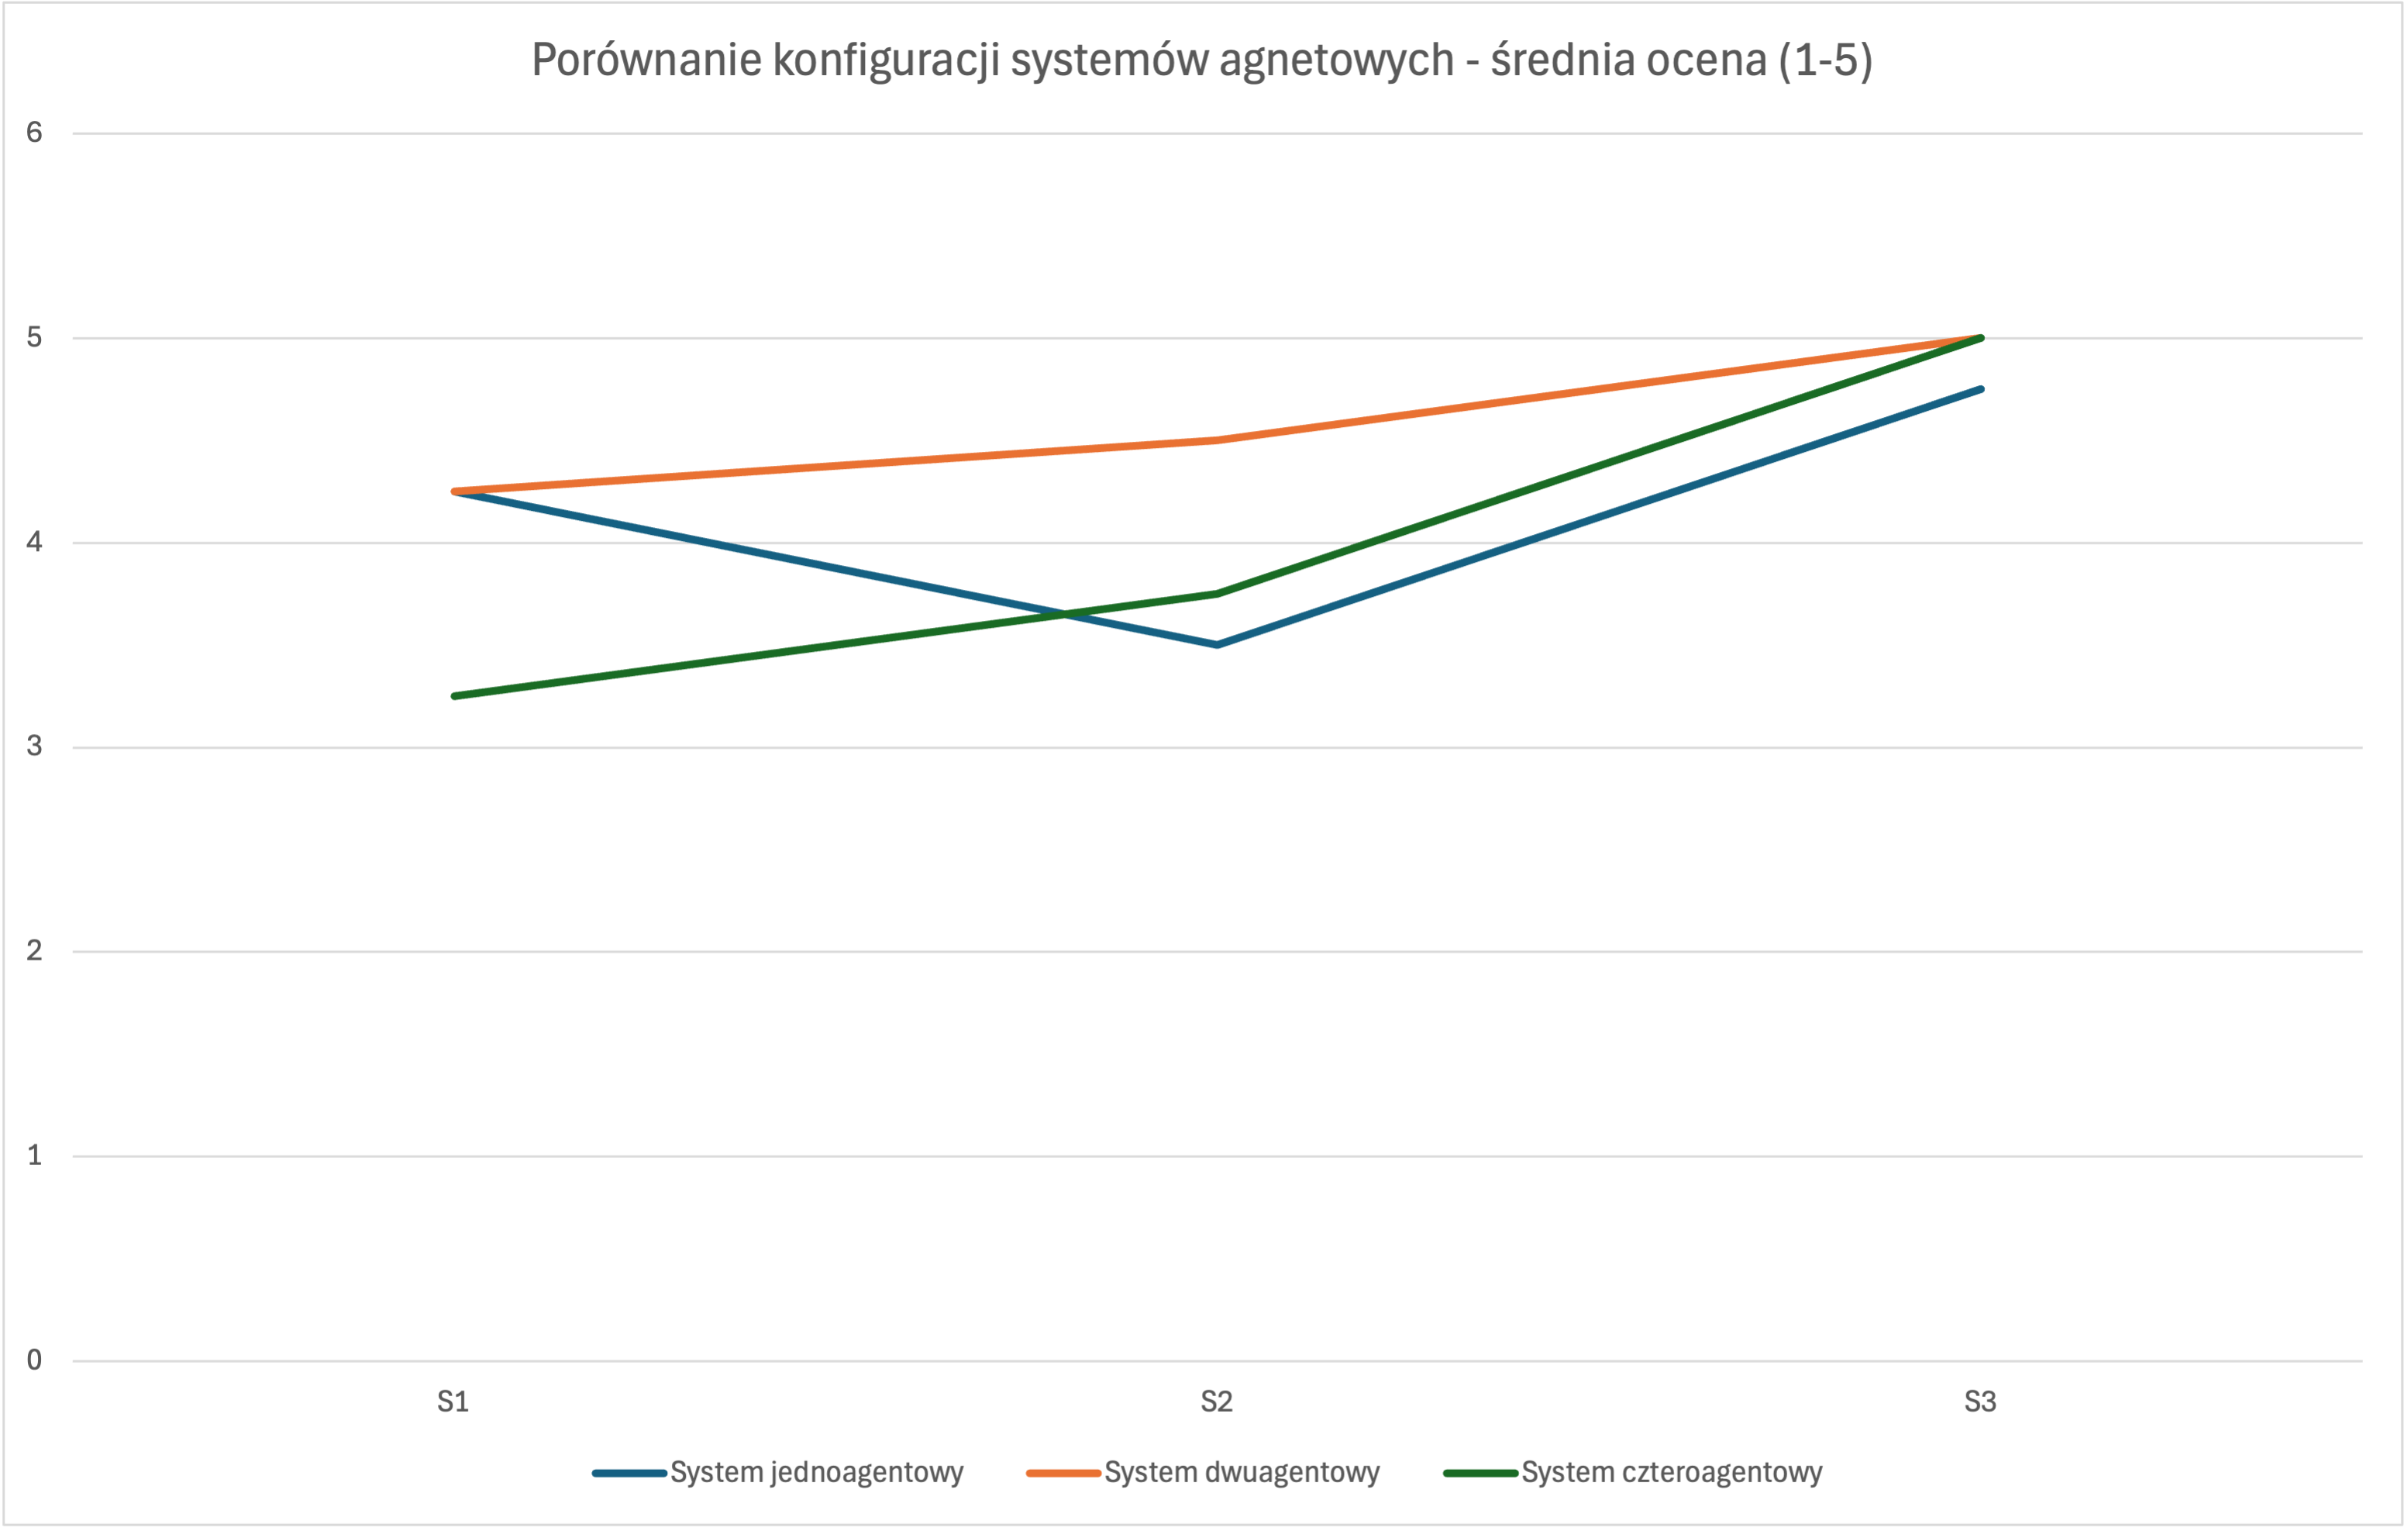
\includegraphics[width=0.9\linewidth]{img/wnioski.png}
    \caption{Uśrednione wyniki scenariuszy dla poszczególnych eksperymentów, inaczej konfiguracji systemu agentowego}
    \label{fig:wnioski-eksperymentów}
\end{figure}

\clearpage